\chapter{Réalisation}
\vspace{5cm}
\large{Ce dernier chapitre présente les spécifications des environnements matériels et logiciels utiliséesau cours du développement et aussi présente les différentes interfaces.\\}


\newpage

\section{les outils et les technologies}

\subsection{Pattern MVC}
Le pattern d'architecture logicielle MVC (\textbf{M}odèle-\textbf{V}ue-\textbf{C}ontrôleur) est un modèle destiné à répondre aux besoins des applications interactives en séparant les problématiques liées aux différents composants au sein de leur architecture respective..
Ce paradigme regroupe les fonctions nécessaires en trois catégories :\\
\begin{itemize}
\item[•] Un modèle : modèle de données.
\item[•] Une vue : interface utilisateur.
\item[•] Un contrôleur : logique de contrôle.\vspace{0.1cm}\\
\end{itemize}

\begin{minipage}{\linewidth}
	\makebox[\linewidth]{
		\includegraphics[keepaspectratio=true,scale=0.45]{mvc10}}
	\captionof{figure}{Pattern MVC.}\label{f3}%    
\end{minipage}\\



\subsection{Outils de développement }
\subsubsection{Langage de programmation}
\begin{minipage}{0.18\textwidth}
	\begin{minipage}{\linewidth}
	\makebox[\linewidth]{
		\includegraphics[keepaspectratio=true,scale=0.4]{jee}} 
		\captionof{figure}{Java EE}\label{f3}%
\end{minipage}
\end{minipage}
\hfill
\begin{minipage}{0.75\textwidth}
(Java Entreprise Edition) est la version entreprise de la plate-forme "Java" qui se compose de l'environnement "JSE" ainsi que de nombreuses API et composants destinés à une utilisation "côté serveur" au sein du système d'information de l'entreprise.\\

\textbf{\textit{Justification:}} JAVA est sécurisée, il a été conçu pour être exploité dans des environnements serveur et distribués. Dans ce cadre, la sécurité n’a pas été négligeable. C’est le langage le plus adopté par les développeurs grâce à sa fiabilité et sa performance élevé. \\
\end{minipage}\\

\subsubsection{Environnement de  développement}
\begin{minipage}{0.2\textwidth}
	\begin{minipage}{\linewidth}
		\makebox[\linewidth]{
			\includegraphics[keepaspectratio=true,scale=0.4]{eclipse.png}} 
			\captionof{figure}{eclipse}\label{f3}%
	\end{minipage}
\end{minipage}
\hfill
\begin{minipage}{0.75\textwidth}
	Eclipse est un environnement de développement intégré pour des applications open source et multi-plateformes. Cela fonctionne principalement comme plateforme de programmation, et il peut compiler et déboguer beaucoup de langues de programmation: bien qu'ils soit plus connu pour la programmation dans Java, sa modularité te permet de l'utiliser pour la programmation en C, Python...\\
	
	\textbf{\textit{Justification:}} Un démarrage rapide et une prise en main progressive,. Un scope fonctionnel complet et une productivité accrue.\\
\end{minipage}\\
\subsubsection{Gestion de version \& collaboration:}
\begin{minipage}{0.2\textwidth}
	\begin{minipage}{\linewidth}
		\makebox[\linewidth]{
			\includegraphics[keepaspectratio=true,scale=0.12]{git}}  
			\captionof{figure}{git}\label{f3}%
	\end{minipage}
\end{minipage}
\hfill
\begin{minipage}{0.75\textwidth}
	Git est un logiciel de gestion de versions décentralisé. C'est un logiciel libre créé par Linus Torvald, auteur du noyau Linux, et distribué selon les termes de la licence publique générale GNU version 2. En 2016, il s’agit du logiciel de gestion de versions le plus populaire qui est utilisé par plus de douze millions de personnes.\\
\end{minipage}\\

\begin{minipage}{0.2\textwidth}
	\begin{minipage}{\linewidth}
		\makebox[\linewidth]{
			\includegraphics[keepaspectratio=true,scale=0.04]{github}} 
			\captionof{figure}{github}\label{f3}%
	\end{minipage}
\end{minipage}
\hfill
\begin{minipage}{0.75\textwidth}
GitHub est un service web d'hébergement et de gestion de développement de logiciels, utilisant le logiciel de gestion de versions Git. Ce site est développé en Ruby on Rails et Erlang par Chris Wanstrath, PJ Hyett et Tom Preston-Werner. GitHub propose des comptes professionnels payants, ainsi que des comptes gratuits pour les projets de logiciels libres. Le site assure également un contrôle d'accès et des fonctionnalités destinées à la collaboration comme le suivi des bugs, les demandes de fonctionnalités, la gestion de tâches et un wiki pour chaque projet.\\
\end{minipage}\\

\subsubsection{Design \& Multimédia:}
\begin{minipage}{0.2\textwidth}
	\begin{minipage}{\linewidth}
		\makebox[\linewidth]{
			\includegraphics[keepaspectratio=true,scale=0.3]{html}}  
			\captionof{figure}{html}\label{f3}%
	\end{minipage}
\end{minipage}
\hfill
\begin{minipage}{0.75\textwidth}
	L'HyperText Markup Language, généralement abrégé HTML, est le langage de balisage conçu pour représenter les pages web. C'est un langage permettant d'écrire de l'hypertexte, d'où son nom.\\
\end{minipage}\\

\begin{minipage}{0.2\textwidth}
	\begin{minipage}{\linewidth}
		\makebox[\linewidth]{
			\includegraphics[keepaspectratio=true,scale=0.04]{css}}
			\captionof{figure}{css}\label{f3}%
	\end{minipage}
\end{minipage}
\hfill
\begin{minipage}{0.75\textwidth}
	Les feuilles de style en cascade, généralement appelées CSS de l'anglais Cascading Style Sheets, forment un langage informatique qui décrit la présentation des documents HTML et XML. Les standards définissant CSS sont publiés par le World Wide Web Consortium.\\
\end{minipage}\\
\begin{minipage}{0.28\textwidth}
	\begin{minipage}{\linewidth}
		\makebox[\linewidth]{
			\includegraphics[keepaspectratio=true,scale=0.31]{js}}   
			\captionof{figure}{JavaScript}\label{f3}%
	\end{minipage}
\end{minipage}
\hfill
\begin{minipage}{0.75\textwidth}
	JavaScript (qui est souvent abrégé en « JS ») est un langage de script léger, orienté objet, principalement connu comme le langage de script des pages web.\\
\end{minipage}\vspace{0.5cm}\\
\begin{minipage}{0.2\textwidth}
	\begin{minipage}{\linewidth}
		\makebox[\linewidth]{
			\includegraphics[keepaspectratio=true,scale=0.18]{eee}}  
			\captionof{figure}{jstl}\label{f3}%
	\end{minipage}
\end{minipage}
\hfill
\begin{minipage}{0.75\textwidth}
	La JavaServer Pages Standard Tag Library est un composant de la plate-forme JEE de développement. Elle étend la spécification JSP en ajoutant une bibliothéque de balises pour les taches courantes, comme le travail sur des fichiers XML, l'exécution conditionnelle, les boucles et l'internationalisation.
\end{minipage}\vspace{0.5cm}\\
\subsubsection{Serveur d’application:}
\begin{minipage}{0.2\textwidth}
	\begin{minipage}{\linewidth}
		\makebox[\linewidth]{
			\includegraphics[keepaspectratio=true,scale=0.31]{tomcat}}   
			\captionof{figure}{Tomcat}\label{f3}%
	\end{minipage}
\end{minipage}
\hfill
\begin{minipage}{0.75\textwidth}
	Tomcat est un conteneur web libre de servlets et JSP. Issu du projet Jakarta, c'est un des nombreux projets de l’Apache Software Foundation.\\
\end{minipage}\\


\section{ Présentation de Louezz}

Cette partie dénombre la présentation des Scénarios applicatifs de l'application. Nous allons présenter dans ce qui suit, les imprimes-écran des principales interfaces réalisées dans notre site web.
\subsection{Page d'accueil}

C'est la page d'accueil qui s'affiche dès l'accès à notre site web, elle est constituée de trois parties principales :\\

• Un champ de recherche donnant aux visiteurs de notre plateforme le choix de sélection des offres selon la ville et la date de disponibilité.\\

• Un slider animé donnant un flash sur les dernieres offres\\



\begin{minipage}{\linewidth}
	\makebox[\linewidth]{
		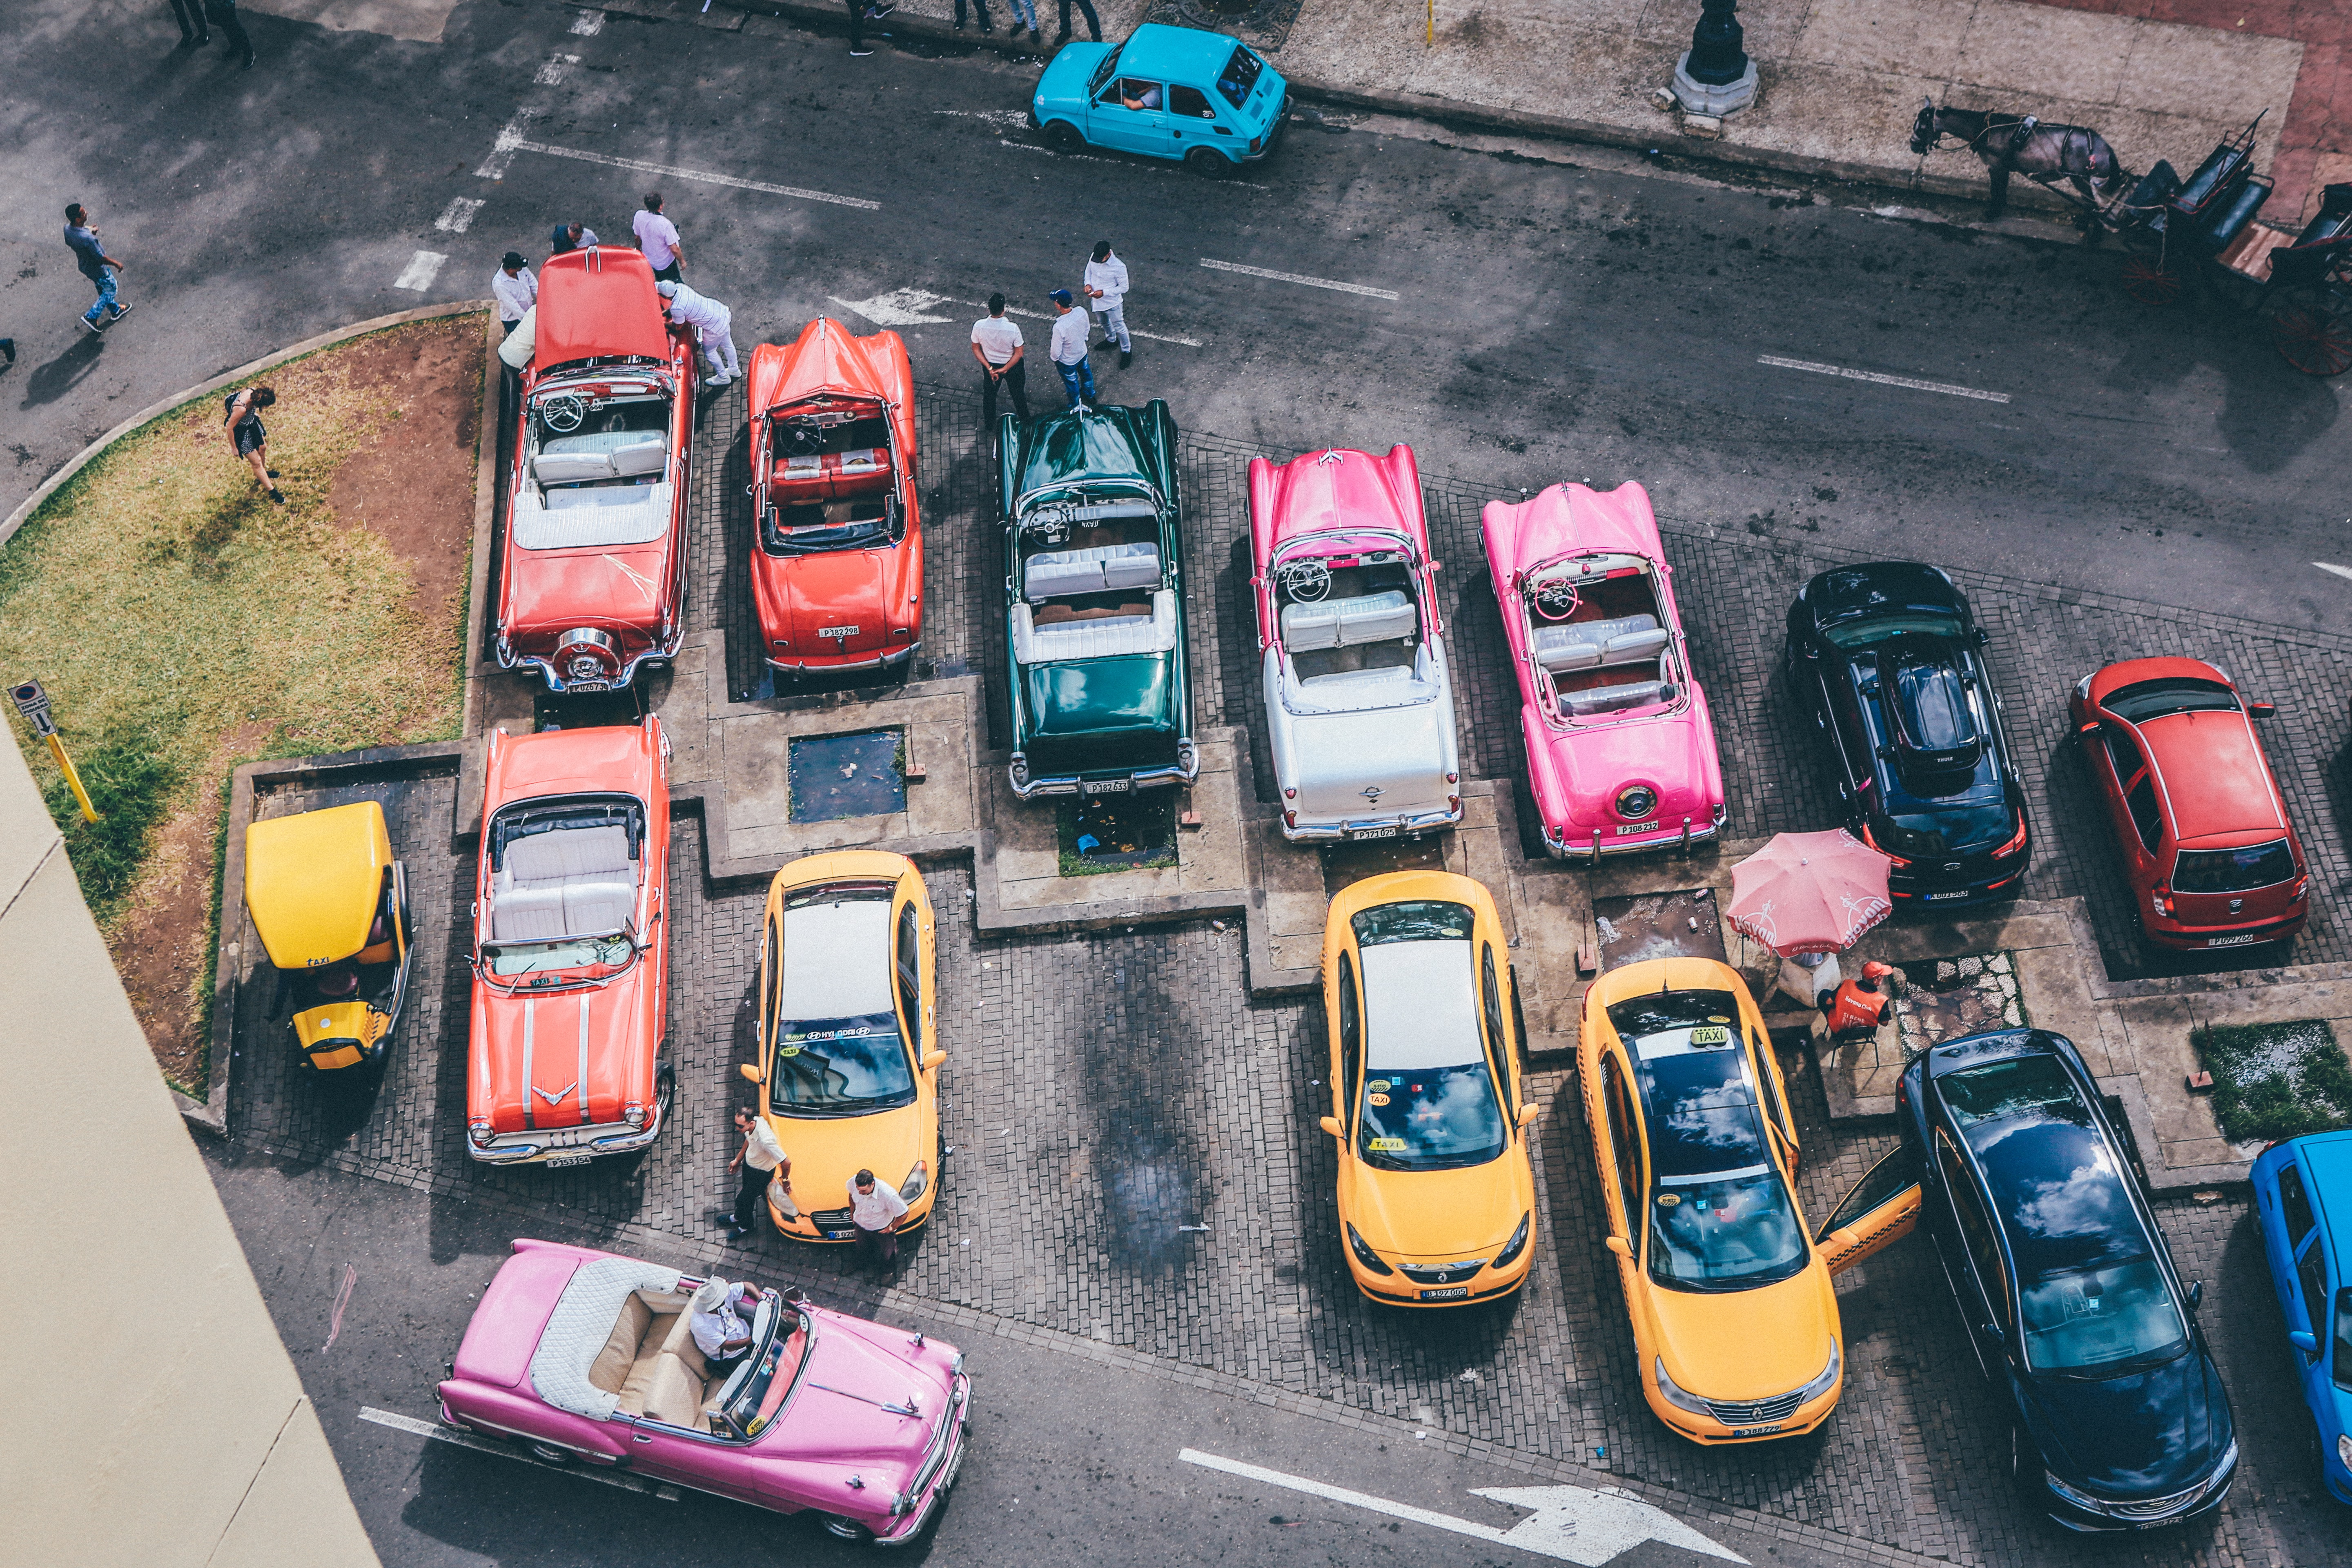
\includegraphics[keepaspectratio=true,scale=0.25]{1.jpeg}}
	\captionof{figure}{Page d'aceuil}\label{f3}%    
\end{minipage}\\


\begin{minipage}{\linewidth}
	\makebox[\linewidth]{
		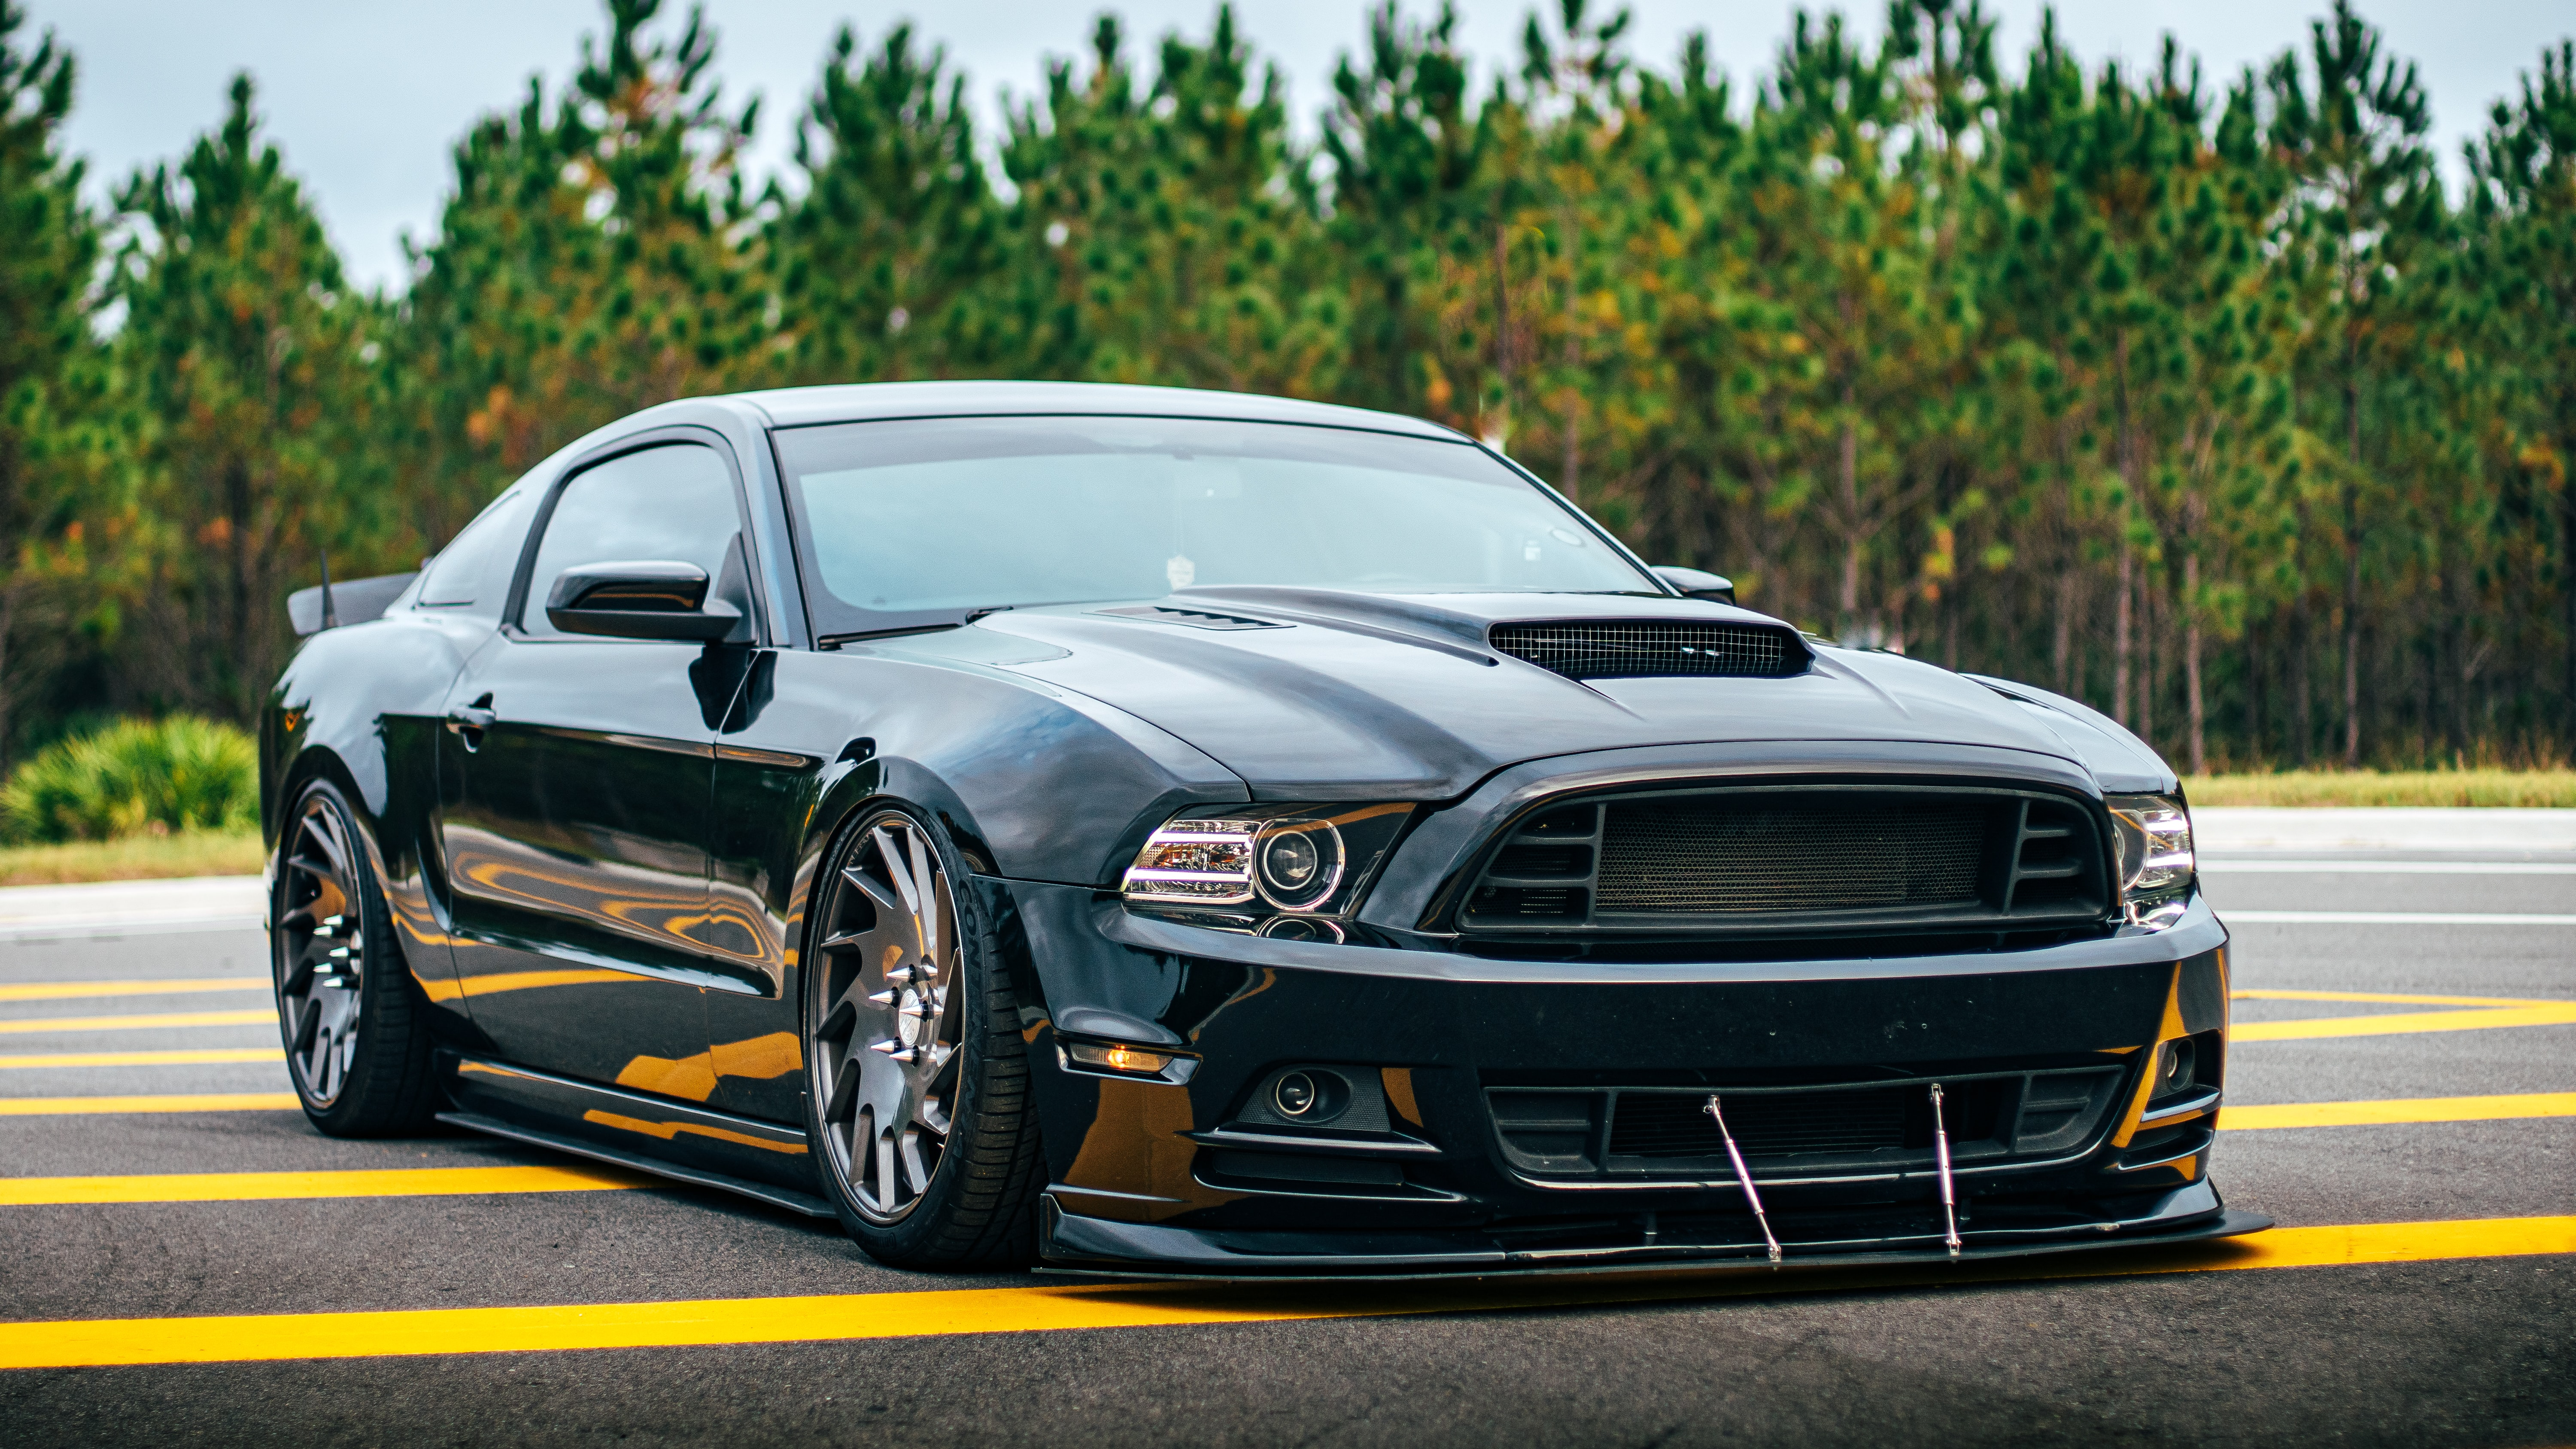
\includegraphics[keepaspectratio=true,scale=0.25]{2.jpeg}}
	\captionof{figure}{Page d'ajout de voiture}\label{f3}%    
\end{minipage}\\


\begin{minipage}{\linewidth}
	\makebox[\linewidth]{
		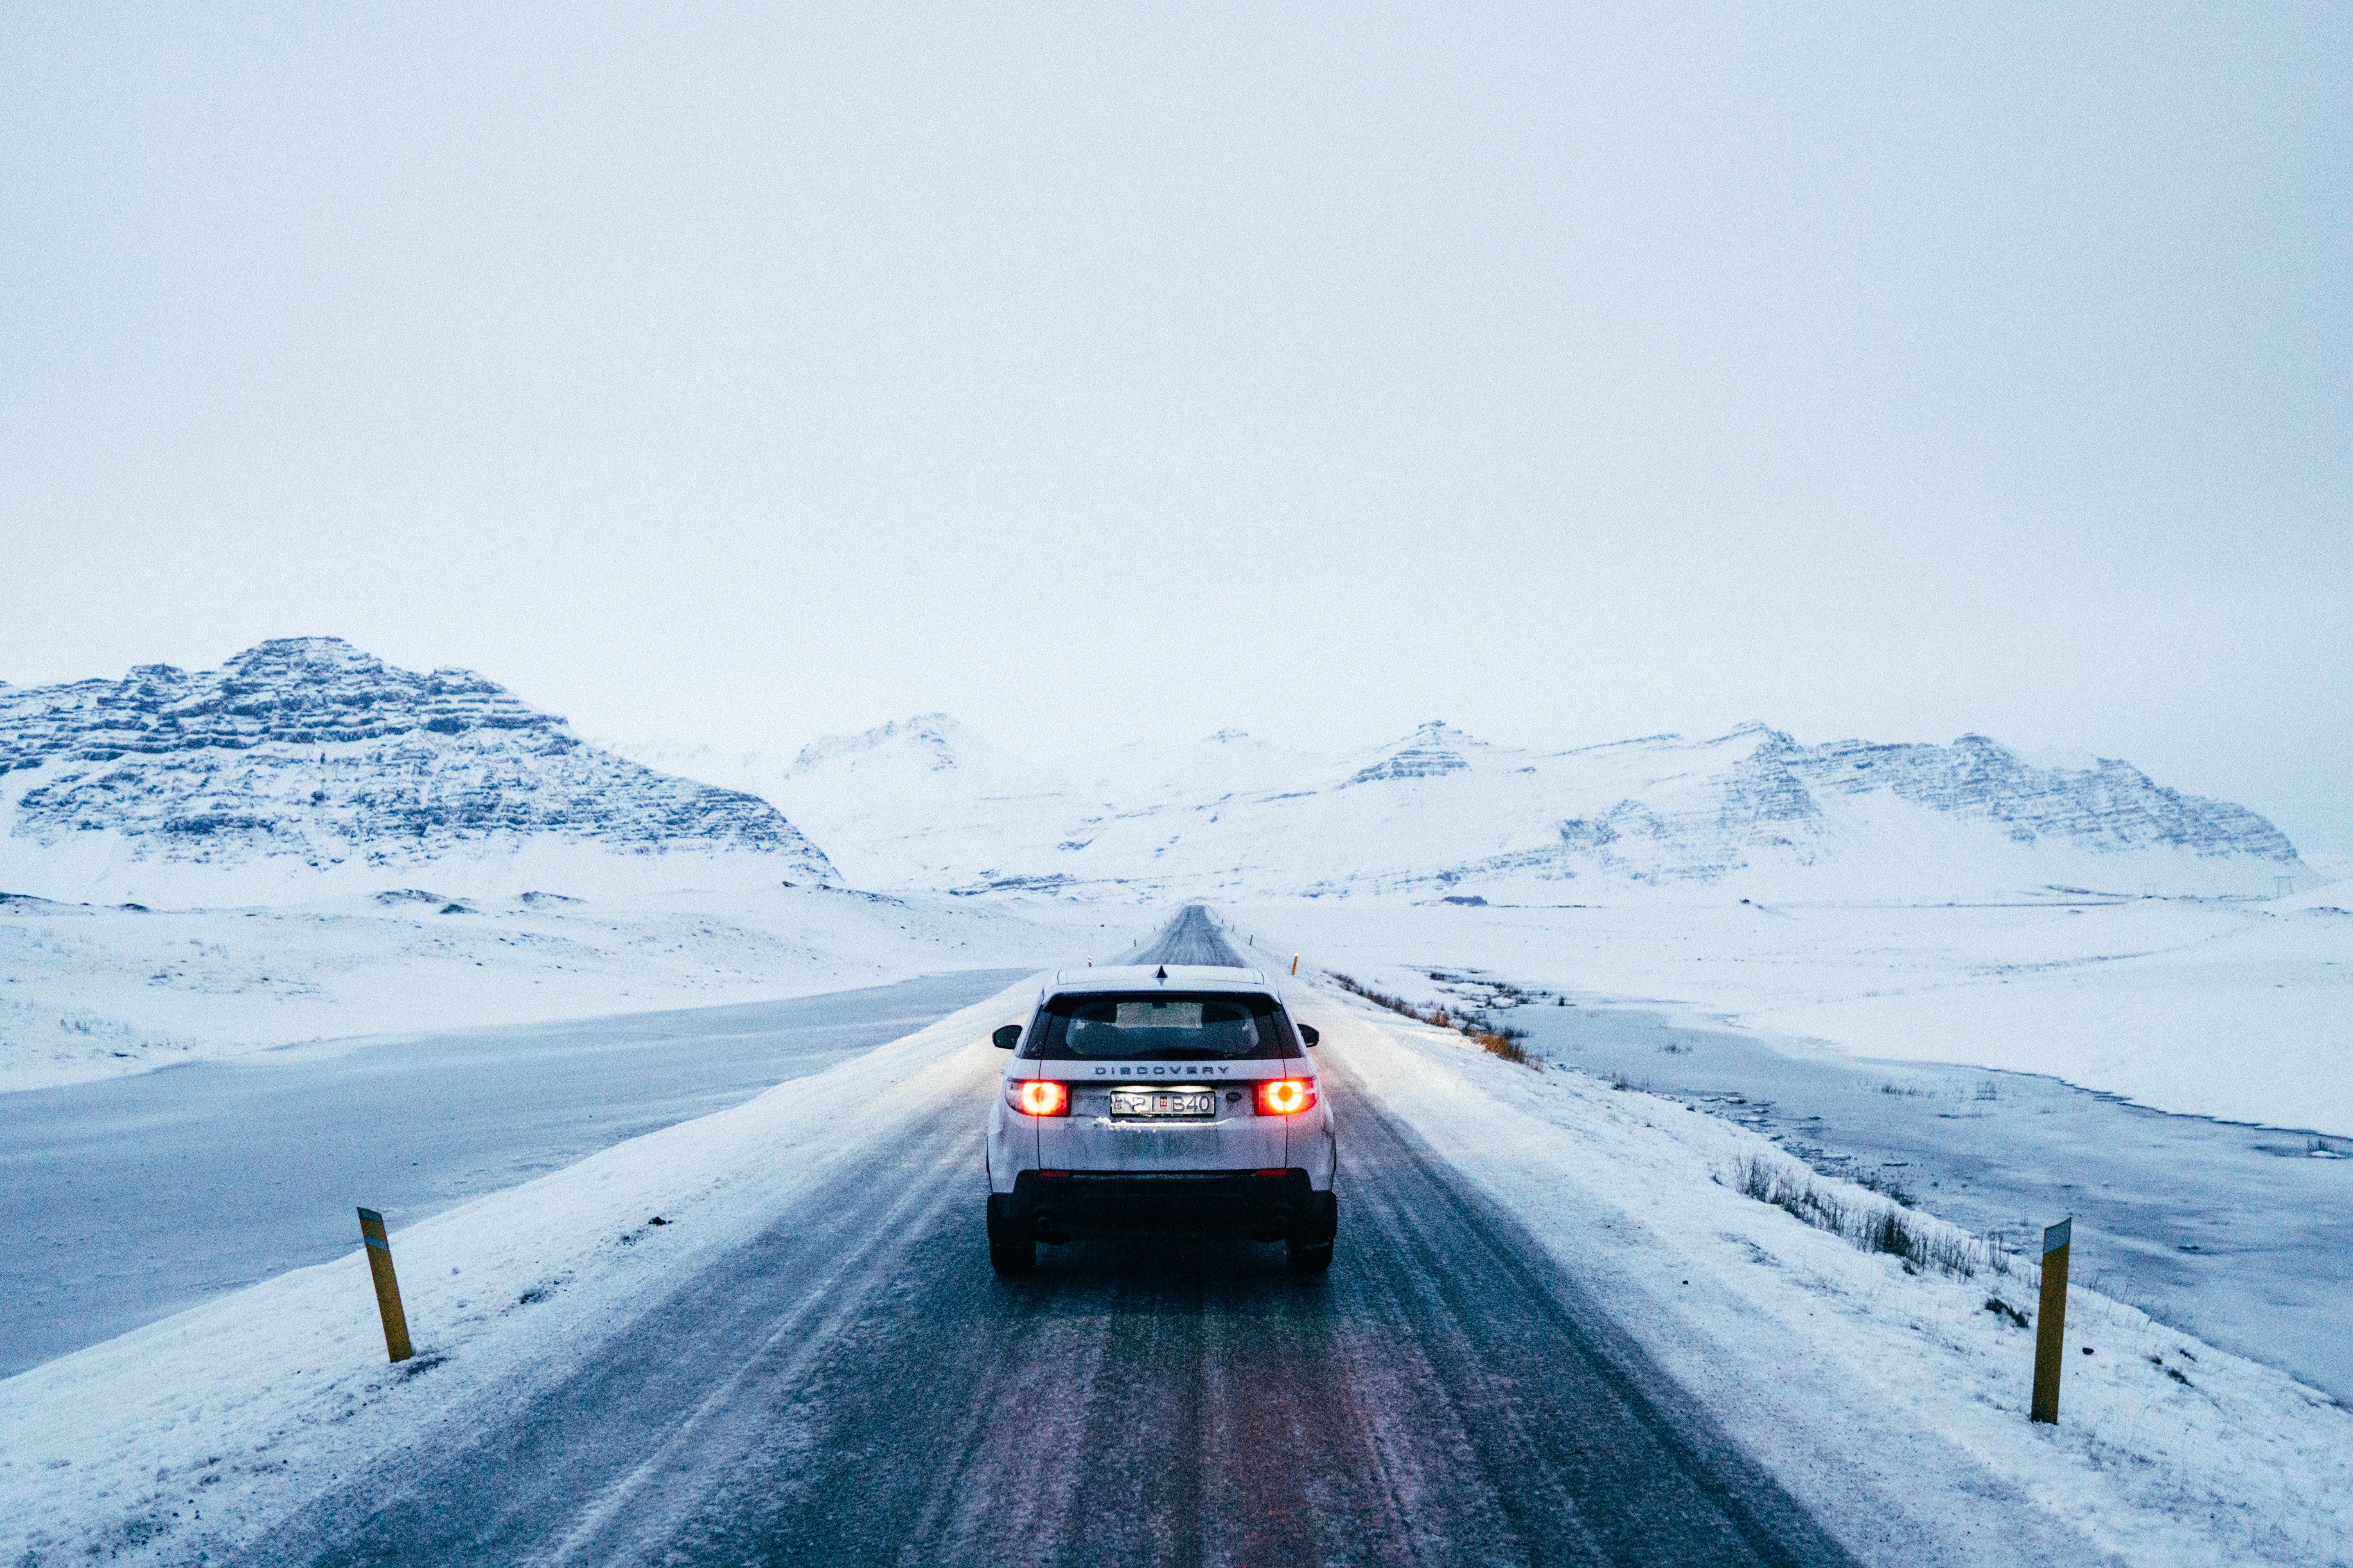
\includegraphics[keepaspectratio=true,scale=0.25]{3.jpeg}}
	\captionof{figure}{Page d'affichage d'offre}\label{f3}%    
\end{minipage}\\


\begin{minipage}{\linewidth}
	\makebox[\linewidth]{
		\includegraphics[keepaspectratio=true,scale=0.25]{4.jpeg}}
	\captionof{figure}{Page de detail d'offfre}\label{f3}%    
\end{minipage}\\

\begin{minipage}{\linewidth}
	\makebox[\linewidth]{
		\includegraphics[keepaspectratio=true,scale=0.25]{5.jpeg}}
	\captionof{figure}{Page de d'affichage de mes voitures}\label{f3}%    
\end{minipage}\\

\begin{minipage}{\linewidth}
	\makebox[\linewidth]{
		\includegraphics[keepaspectratio=true,scale=0.25]{6.jpeg}}
	\captionof{figure}{Page de modification des donnees de ma voiture}\label{f3}%    
\end{minipage}\\

\begin{minipage}{\linewidth}
	\makebox[\linewidth]{
		\includegraphics[keepaspectratio=true,scale=0.25]{7.jpeg}}
	\captionof{figure}{Page de profile}\label{f3}%    
\end{minipage}\\

\begin{minipage}{\linewidth}
	\makebox[\linewidth]{
		\includegraphics[keepaspectratio=true,scale=0.25]{8.jpeg}}
	\captionof{figure}{Page de changement de mot de passe}\label{f3}%    
\end{minipage}\\

\begin{minipage}{\linewidth}
	\makebox[\linewidth]{
		\includegraphics[keepaspectratio=true,scale=0.25]{9.jpeg}}
	\captionof{figure}{  Page de modification des données de mon profile}\label{f3}%    
\end{minipage}\\
\begin{minipage}{\linewidth}
	\makebox[\linewidth]{
		\includegraphics[keepaspectratio=true,scale=0.25]{11.jpeg}}
	\captionof{figure}{  Page de connexion}\label{f3}%    
\end{minipage}\\


\begin{minipage}{\linewidth}
	\makebox[\linewidth]{
		\includegraphics[keepaspectratio=true,scale=0.25]{12.jpeg}}
	\captionof{figure}{  Page d'inscription}\label{f3}%    
\end{minipage}\\

\begin{minipage}{\linewidth}
	\makebox[\linewidth]{
		\includegraphics[keepaspectratio=true,scale=0.25]{13.jpeg}}
	\captionof{figure}{
	Page de demandes ou cas d'inexistance des demandes
	}\label{f3}%    
\end{minipage}\\

\begin{minipage}{\linewidth}
	\makebox[\linewidth]{
		\includegraphics[keepaspectratio=true,scale=0.25]{14.jpeg}}
	\captionof{figure}{Page de mes voitures
	
	}\label{f3}%    
\end{minipage}\\

\begin{minipage}{\linewidth}
	\makebox[\linewidth]{
		\includegraphics[keepaspectratio=true,scale=0.25]{15.jpeg}}
	\captionof{figure}{Page de done}\label{f3}%    
\end{minipage}\\

\begin{minipage}{\linewidth}
	\makebox[\linewidth]{
		\includegraphics[keepaspectratio=true,scale=0.25]{10.jpeg}}
	\captionof{figure}{Page des erreurs}\label{f3}%    
\end{minipage}\\